%
% Kapitel1.tex 
%
\chapter{Introduction}

Perimeter monitoring is a cornerstone of modern security and surveillance of a location. A powerful technology for this application is Digital Acoustic Sensing (DAS)~\cite{duckworth}, which effectively transforms long stretches of fibre optic cable into a continuous array of highly sensitive microphones. These systems capture detailed acoustic data by measuring minute phase shifts in light traveling through the fibre, enabling the real-time detection of ground vibrations caused by various activities.

This thesis focuses on activities relevant to perimeter security, such as walking, climbing, or vehicle movement, as conceptually illustrated in the theoretical airport security layout in Figure~\ref{Airport}. In such a scenario, a DAS system, with fiber optic cables indicated by the red lines, would be deployed to monitor the entire perimeter for potential intrusions.

\begin{figure}[h]
    \centering
    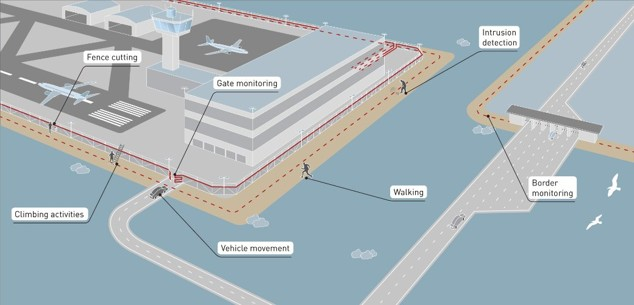
\includegraphics[width=\linewidth]{Bilder/jpg/Airport.jpg}
    \caption{A theoretical perimeter monitoring setup at an airport~\cite{Airport_Image}.}
    \label{Airport}
\end{figure}

While DAS provides a wealth of raw data, interpreting this data to reliably identify specific events is a significant challenge. To address this, this thesis presents the spectrogram classifier framework, a complete pipeline designed to detect and classify human footsteps from raw DAS phase data. The research presented was conducted in collaboration with AP Sensing, who provided the DAS system (Figure~\ref{System}) and associated software used for data acquisition.

The core of the framework first transforms raw, one-dimensional DAS phase data into two-dimensional time-frequency representations called spectrograms. These spectrograms, which visually resemble images, are then fed into modern deep learning vision networks for classification. This approach leverages the advanced pattern-recognition capabilities of convolutional neural networks (CNNs) to distinguish between ambient noise and the unique signatures of footsteps.

\begin{figure}[h]
    \centering
    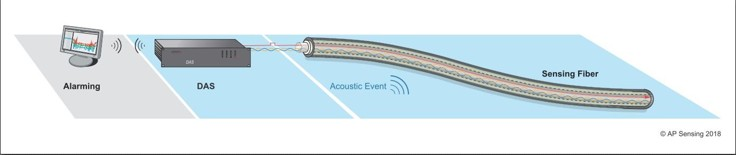
\includegraphics[width=\linewidth]{Bilder/jpg/System.jpg}
    \caption{DAS setup~\cite{DAS_PPT}.}
    \label{System}
\end{figure}

To validate the framework and determine the most effective configuration, this thesis evaluates two state-of-the-art vision models: ConvNeXt V2~\cite{liu2023convnextv2} and EfficientNet~\cite{tan2019efficientnet}. The performance of these models is rigorously tested by training and evaluating them on a custom dataset of walking patterns. By comparing their accuracy, false alarm rates, and real-time performance, this work identifies the optimal model and data configuration for a field-ready perimeter monitoring tool. Ultimately, this thesis demonstrates the efficacy of the Spectrogram Classifier Framework as a robust and reliable solution for security surveillance applications.